\subsection{Тестирование разработанного программно-аппаратного комплекса}

\subsubsection{Получение данных о состоянии комплекса}

Для тестирования разработанного программно-аппаратного комплекса использовалось разработанное веб-приложение.

В первую очередь необходимо определить, достоверную ли предоставляет информацию сервер программно-аппаратного комплекса. При запуске работы системы включается сервер, проверяется, подключен ли к системе микрофон, а так же запускается процесс отображения цветов на светодиодной ленте. Также устанавливаются начальные значения яркости свечения светодиодов, скорость передвижения светодиодов по ленте, а также нижняя граница звучания звука и максимальный процент зашумлённости звука. Яркость свечения светодиодов при этом устанавливается в максимальное значение (255), так же как и скорость передвижения светодиодов по ленте (60). Нижняя граница звучания звука и максимальный процент зашумлённости устанавливаются вне зависимости от подключения микрофона и равны, соответственно, 127 (среднее значение) и 0,4.

На рисунке~\ref{img:test__home-on} представлена проверка корректности полученных от сервера данных о состоянии комплекса. Зеленому кругу справа от названия типа данных соответствует активное подключение, а красному -- отключенное.

\begin{figure}[H]
  \centering
  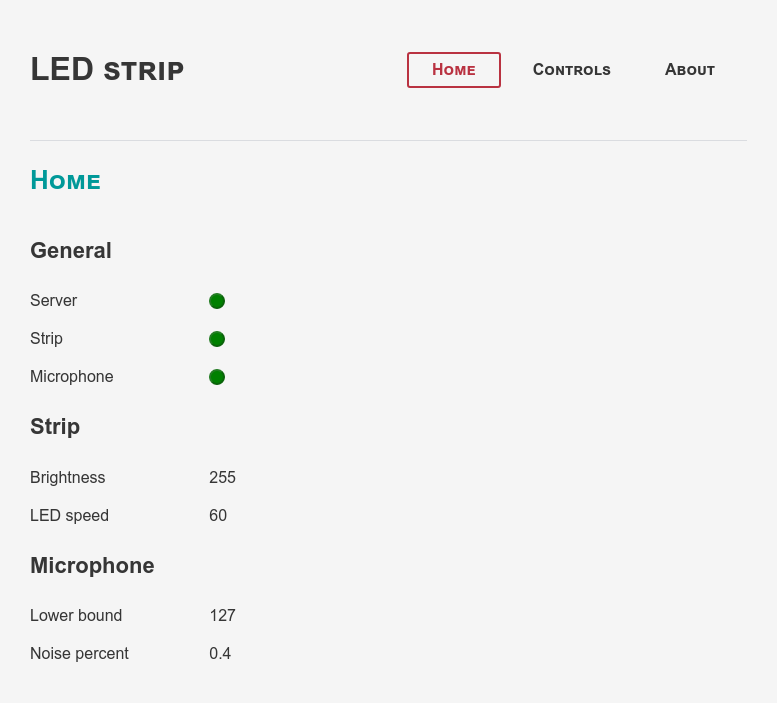
\includegraphics[height=0.3\textheight]{assets/images/practical/test__home-on.png}
  \caption{Полученные от сервера данные о состоянии комплекса}
  \label{img:test__home-on}
\end{figure}

При этом на светодиодной ленте отображается эффект бегущих из центра огней, цвет которых определяется звуком, поступающим на микрофон. На рисунке~\ref{img:test__state1} представлено поведение светодиодной ленты.

\begin{figure}[H]
  \centering
  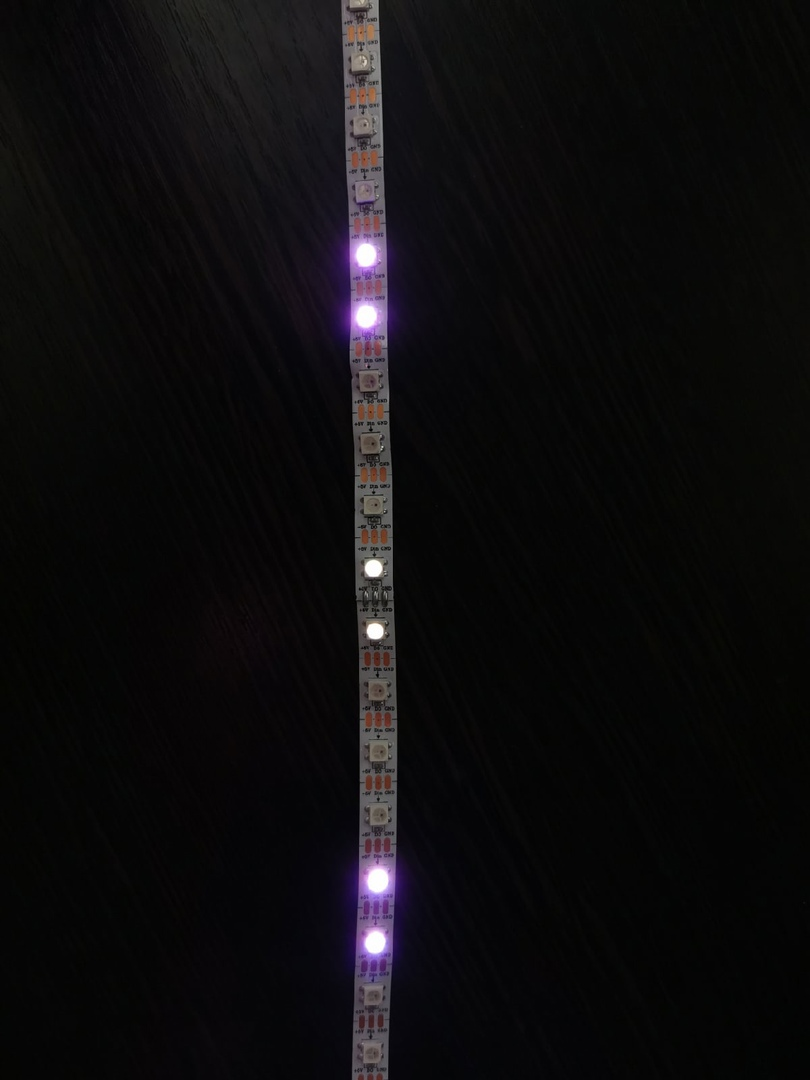
\includegraphics[angle=90, height=0.3\textheight]{assets/images/practical/test__state1.jpg}
  \caption{Начальное поведение светодиодной ленты}
  \label{img:test__state1}
\end{figure}

При отключении микрофона сервер также предоставляет корректные данные (рисунок~\ref{img:test__home-off}).

\begin{figure}[H]
  \centering
  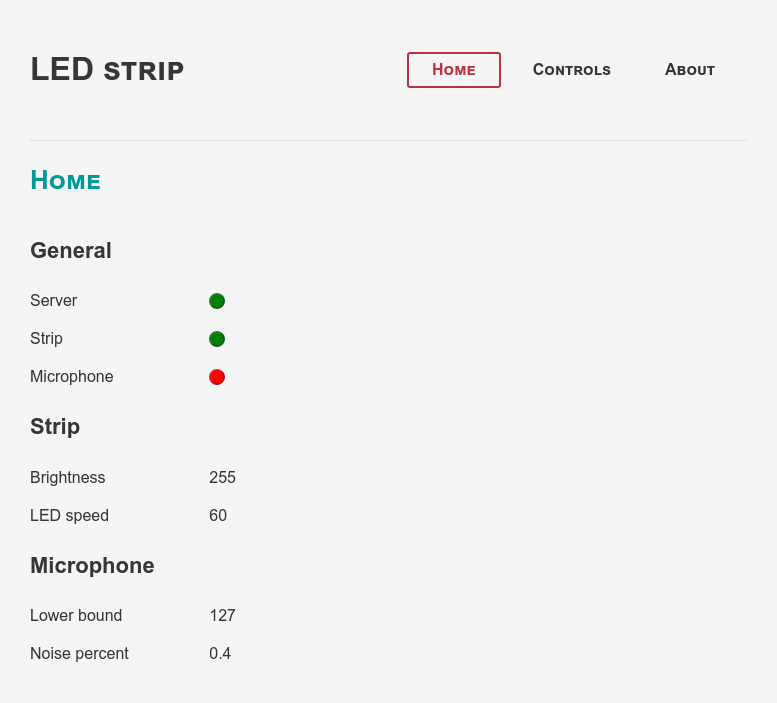
\includegraphics[height=0.3\textheight]{assets/images/practical/test__home-off.png}
  \caption{Состоянии комплекса при отключении микрофона}
  \label{img:test__home-off}
\end{figure}

\subsubsection{Изменение состояния комплекса}

На странице управления состоянием комплекса с помощью переключателей можно:

\begin{enumerate}
  \item Включить/выключить светодиодную ленту;
  \item включить/выключить микрофон;
  \item задать значение яркости свечения;
  \item задать скорость перемещения светодиодов;
  \item указать нижняя граница звучания звука;
  \item указать максимальный процент зашумлённости.
\end{enumerate}

При выключении светодиодной ленты с помощью веб-приложения, светодиоды на светодиодной ленте перестают отображаться. На рисунке~\ref{img:test__controls-strip-off} представлен страница управления комплексом при выключении светодиодной ленты.

\begin{figure}[H]
  \centering
  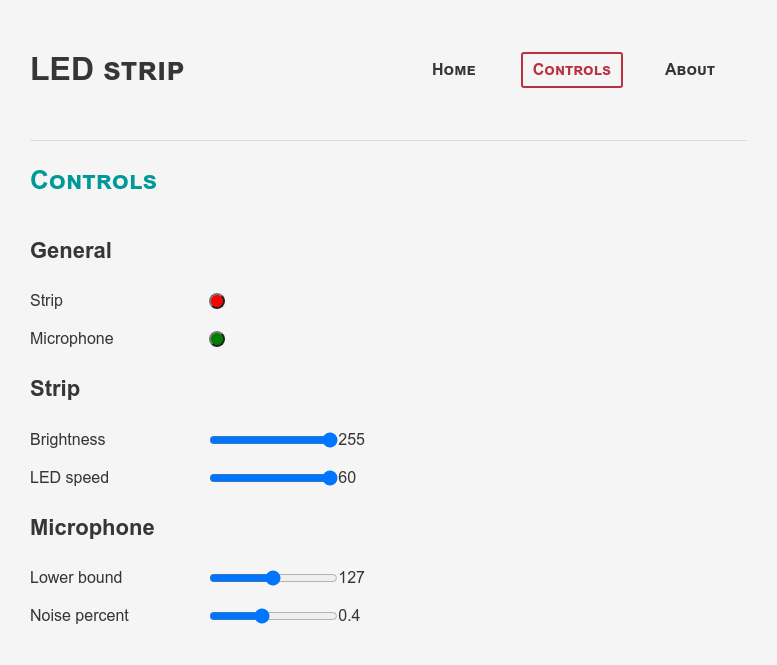
\includegraphics[height=0.3\textheight]{assets/images/practical/test__controls-strip-off.png}
  \caption{Выключение светодиодной ленты с помощью веб приложения}
  \label{img:test__controls-strip-off}
\end{figure}

Также можно изменить яркость свечения светодиодов, установив значение яркости в веб приложении. На рисунке~\ref{img:test__controls-brightness-60} представлена установка значения яркости в 60, на рисунке~\ref{img:test__state2} -- поведение светодиодной ленты при установке этого значения.

\begin{figure}[H]
  \centering
  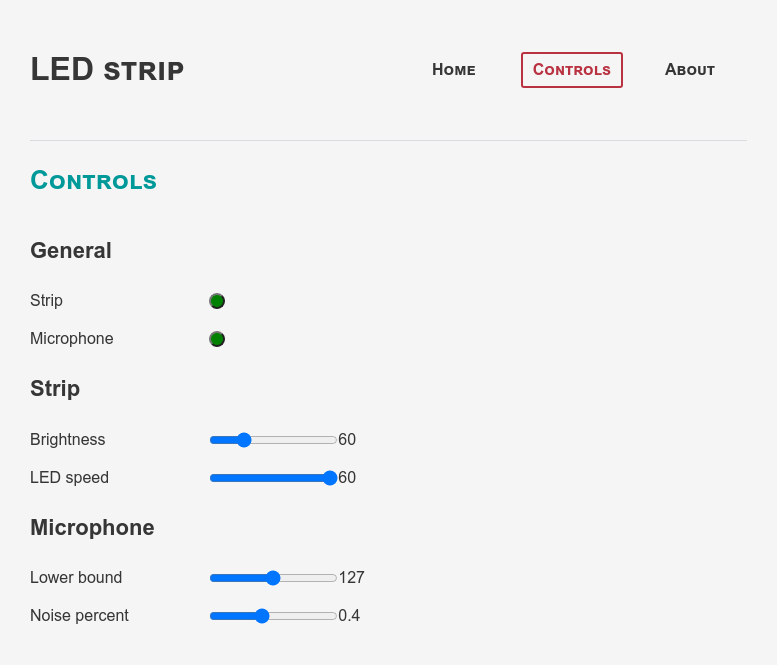
\includegraphics[height=0.3\textheight]{assets/images/practical/test__controls-brightness-60.png}
  \caption{Установка яркости свечения светодиодов в веб приложении}
  \label{img:test__controls-brightness-60}
\end{figure}

\begin{figure}[H]
  \centering
  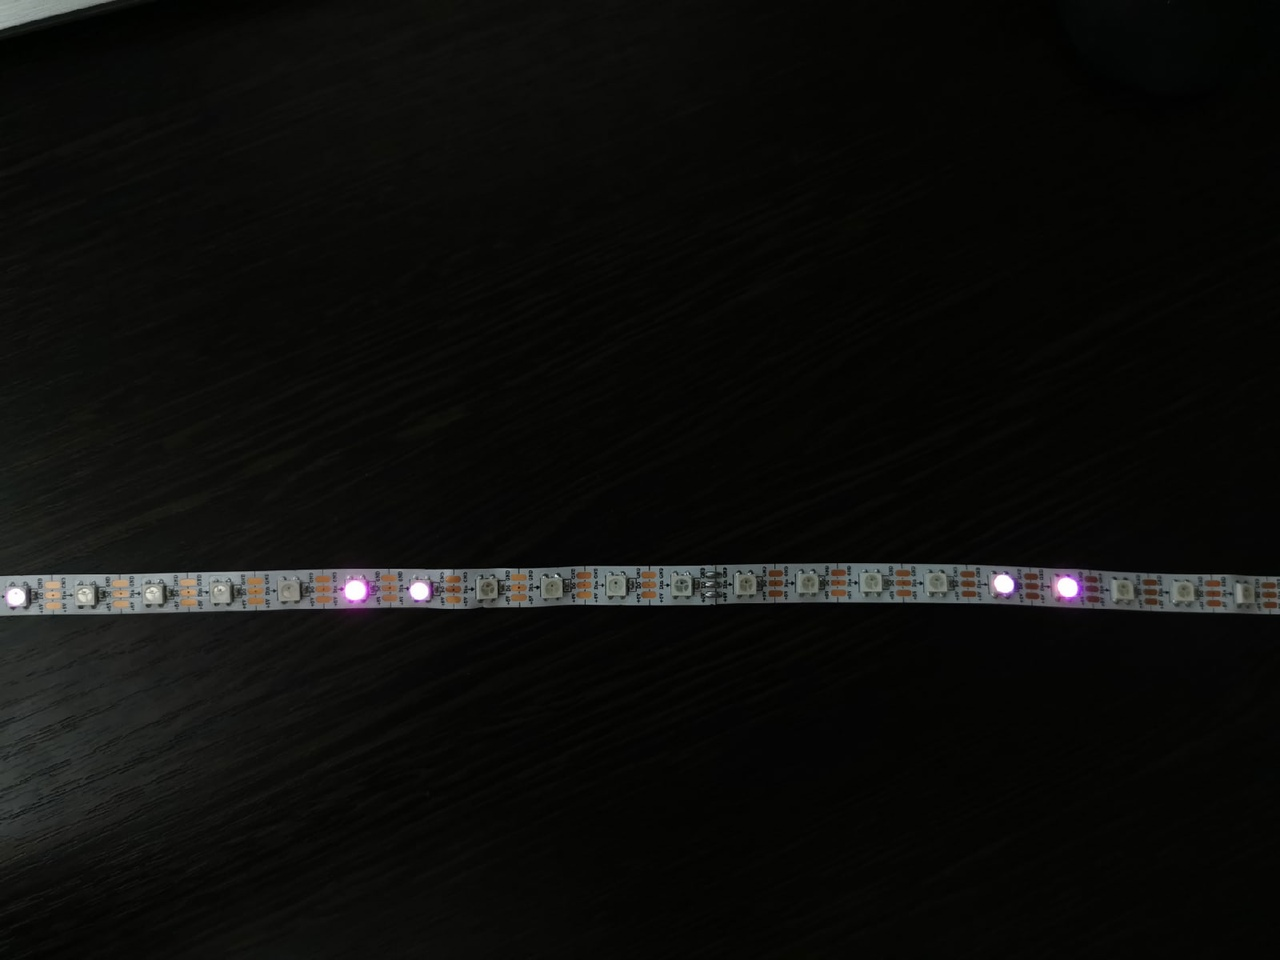
\includegraphics[height=0.25\textheight]{assets/images/practical/test__state2.jpg}
  \caption{Поведение светодиодной ленты при установке яркости равной 60}
  \label{img:test__state2}
\end{figure}

При уменьшении максимального значения зашумлённости эффект бегущих из центра огней становится более редким, так как при обработке звука происходит более тщательная фильтрация шумов. На рисунке~\ref{img:test__controls-noise-01} представлена установка максимального значения зашумлённости равным 10\% (0.1).

\begin{figure}[H]
  \centering
  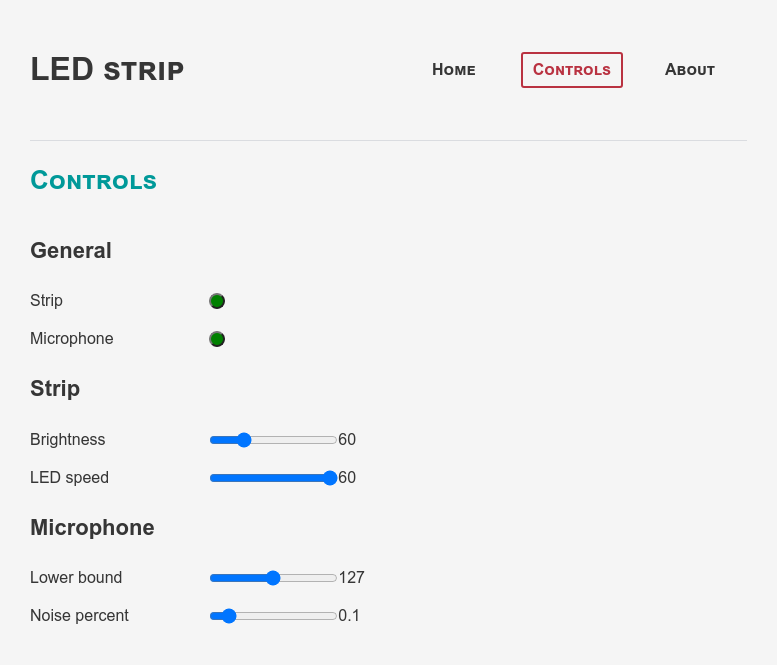
\includegraphics[height=0.3\textheight]{assets/images/practical/test__controls-noise-01.png}
  \caption{Установка максимального значения зашумлённости в веб приложении}
  \label{img:test__controls-noise-01}
\end{figure}

Также были протестированы изменения в поведении комплекса при изменении оставшихся переключателей. Во всех тестах изменение поведения комплекса было ожидаемым и корректным, что показывает эффективность и работоспособность разработанного программно-аппаратного комплекса.
